\documentclass[aspectratio=169,t,11pt,table]{beamer}
\usepackage{../includes/slides,../includes/math}
\definecolor{accent}{HTML}{2B5269}
\definecolor{accent2}{HTML}{9D2235}

\title{Regression Methods}
\subtitle{\it  ECON 5753 — University of Arkansas}
\date{Sprint 2025}
\author{Prof. Kyle Butts}

\NewDocumentCommand{\logistic}{o g}{%
  \textrm{logistic}\IfValueT{#1}{_{#1}}{\left(#2\right)}
}

\begin{document}

% ------------------------------------------------------------------------------
\begin{frame}[noframenumbering,plain]
\maketitle
\end{frame}
% ------------------------------------------------------------------------------

\section{Introduction to Time-Series}

\begin{frame}{Time-series}
  \alert{Time-series} data is a set of observations $y_t$ that occur for a single unit measured over the course of time
  \begin{itemize}
    \item In general, we call $t$ the `period'
    
    \medskip
    \item If the time-series is spaced evenly over time without missing, it is called \alert{regular}. 
    \begin{itemize}
      \item Some methods require regular time intervals, and will do weird things if you give it irregular time series
    \end{itemize}
    
    \medskip
    \item If you observe many units' time-series, this is called \alert{panel data}
    \begin{itemize}
      \item Panel data that is regular is called a \alert{balanced panel}
    \end{itemize}
  \end{itemize}
\end{frame}

\begin{frame}{Examples}
  Examples include:
  \begin{itemize}
    \item Annual data on the DGP of a country
    \item Hourly stock price for a company
    \item Annual data on cigarette consumption per capita in a state 
    \item A sport's teams number of points scored in games (unequally spaced)
  \end{itemize}

  \bigskip
  For each example, think through:
  \begin{enumerate}
    \item Is this a regular time-series?
    
    \item Is this a panel dataset?
  \end{enumerate}
\end{frame}

\imageframe{figures/unemployment_rate.pdf}
\imageframe{figures/arkansas_2023_football.pdf}
\imageframe{figures/apple_stock.pdf}
% \imageframe{figures/smoking_california.pdf}
\imageframe{figures/smoking_a_few_states.pdf}

\begin{frame}{What is special about time-series?}
  In our previous topics, we have been thinking about \alert{cross-sectional} data
  \begin{itemize}
    \item Each person in your dataset is an independent draw that provides us with unique information
  \end{itemize}

  \bigskip
  In cross-sectional data, knowing about one indivdiual does not really tell me much information about another
  \begin{itemize}
    \item This is not \emph{entirely true}; e.g. worker's in same firm have common experiences, kids in same school have same teacher quality, etc. (hence why we might cluster our standard errors)
  \end{itemize}
\end{frame}

\begin{frame}{What is special about time-series?}
  In time-series data, knowing last period's value of $y_{t-1}$ is often very useful for this period's value of $y_{t}$
  \begin{itemize}
    \item This property is essential in forecasting; following a variable over time might let us predict future values
    
    \item Shocks that happened last period probably still impact me today(!) 
  \end{itemize}

  \pause
  \bigskip
  Another way of saying this, is if we randomly shuffled time-series data, we would lose information!
  \begin{itemize}
    \item This is not true of a cross-sectional dataset; we can reshuffle rows without problem 
  \end{itemize}
\end{frame}

\imageframe{figures/unemployment_rate.pdf}
\imageframe{figures/unemployment_rate_rand_shuffle.pdf}

\begin{frame}{Thinking about inference with time-series}
  We have a bit of a problem with our time-series:
  $$
    y_1, y_2, \dots, y_T
  $$
  \vspace*{-\bigskipamount}
  \begin{itemize}
    \item $y_1$ is related to $y_2$ 
    \item $y_2$ is related to $y_3$
    \item and so on...
  \end{itemize}

  \bigskip
  In some sense, we have only a `single' observation 
\end{frame}

\imageframe{figures/time_series_sampling_orig.pdf}
\imageframe{figures/time_series_sampling_extra_sample_1.pdf}
\imageframe{figures/time_series_sampling_extra_sample_2.pdf}
\imageframe{figures/time_series_sampling_extra_sample_5.pdf}
\imageframe{figures/time_series_sampling_and_mu.pdf}

\begin{frame}{Thinking about inference with time-series}
  \vspace*{-\bigskipamount}
  $$
    y_1, y_2, \dots, y_T
  $$
  
  \bigskip
  While every observation might be related to one another, we are typically willing to assume that as you move away in time, observations become less and less correlated.
  

  % TODO: golden rule of time-series (golden rule of spatial statistics)
  \begin{tcolorbox}[boxrule = 0pt, frame hidden, sharp corners, enhanced, borderline west = {2pt}{0pt}{blue}, interior hidden]
    ``''
  \end{tcolorbox}
\end{frame}

\begin{frame}{Thinking about inference with time-series}
  \vspace*{-\bigskipamount}
  $$
    y_1, y_2, \dots, y_T
  $$
  
  Hence, statistical inference is quite a bit more challenging in time-series and requires weak dependency central limit theorems
  \begin{itemize}
    \item The intuition is that as you have larger and larger $T$, the information you have increases
  \end{itemize}

  \pause
  \bigskip
  But, we will not spend much time discussing that in this class:
  \begin{itemize}
    \item If you are running time-series regressions, default to Newey West standard errors; in \texttt{fixest}, use \texttt{vcov = NW(lag = \#)}
  \end{itemize}
\end{frame}


\section{Learning from Time-Series}

\begin{frame}{What we can gain from using time-series}
  Time-series forecasting can be useful to:
  \begin{itemize}
    \item Predict future values based on past data

    \item Inform decision-making by anticipating changes over time

    \item Identify patterns like trends or seasonality
  \end{itemize}
\end{frame}

\begin{frame}{Two goals of time-series}
  There are two possible goals that we can tackle when working with time-series data:
  \begin{enumerate}
    \item Learn about \emph{persistent} patterns in how $y_t$ evolves over time while ignoring random fluctuations (inference)
    \begin{itemize}
      \item E.g. learn about seasonality, trends, etc.
    \end{itemize}
    
    \medskip
    \item Predict future values of $y_t$ (forecasting)
    \begin{itemize}
      \item The above step might be useful in predicting future $y$, but not necessary (only care about prediction)
    \end{itemize}
  \end{enumerate}

  \bigskip
  Will try to clarify when we are discussing forecasting vs. describing time-series patterns (inference)
\end{frame}

\begin{frame}{Learning from time-series}
  We observe a set of time-series observations $y_t$. Think of the observed $y$ as being generated by 
  $$
    y_t = {\color[HTML]{B3114B} \mu_t} + \varepsilon_t
  $$
  \begin{itemize}
    \item ${\color[HTML]{B3114B} \mu_t}$ is the `typical' or `systematic' value of $y$ at time $t$
    
    \item $\varepsilon_t$ is a random fluctuation
  \end{itemize}

  \bigskip
  Of course, we do not know which fluctuations are due to $\mu_t$ changing over time or $\varepsilon_t$ changing over time
  \begin{itemize}
    \item Without any more structure, this is is an impossible task
  \end{itemize}
\end{frame}

\begin{frame}{Learning from time-series}
  \vspace*{-\bigskipamount}
  $$
    y_t = {\color[HTML]{B3114B} \mu_t} + \varepsilon_t
  $$

  Say we assume $\expec{\varepsilon_t} = 0$
  \begin{itemize}
    \item On average over different draws of the time-series, the error term is on average 0
  \end{itemize}

  \bigskip
  But, our observed time-series is a single draw, so it's not obvious that the noise will `average away'
  \begin{itemize}
    \item Is the bump in the time-series just a shock that affected the unit for multiple periods or a systematic component
  \end{itemize}
\end{frame}

\begin{frame}{Learning from time-series}
  \vspace*{-\bigskipamount}
  $$
    y_t = {\color[HTML]{B3114B} \mu_t} + \varepsilon_t
  $$

  \bigskip
  Two options for solving this:
  \begin{enumerate}
    \item Assume that $\varepsilon_t$ is not too persistent, and use some kind of `smoothing' method to smooth out noise
    
    \item Rely on functional form assumptions and run a time-series regression 
    \begin{itemize}
      \item By pooling over time, we are averaging out noise (but requires us to model ${\color[HTML]{B3114B} \mu_t}$ well)
    \end{itemize}
  \end{enumerate}
\end{frame}

\imageframe{figures/time_series_sampling_and_mu.pdf}

\begin{frame}{}
  $$
    y_t = {\color[HTML]{B3114B} \mu_t} + \varepsilon_t
  $$
  
  Here are some examples of what we can hope to learn using time-series data:
  \begin{enumerate}
    \item Identify \alert{seasonality} in data 
    \begin{itemize}
      \item Does the change in ${\color[HTML]{B3114B} \mu_t}$ over the year follow a standard pattern?
      \item E.g. retail sales increasing in December
    \end{itemize}
    
    \medskip
    \item Detect long-term \alert{trends} and \alert{short-term shocks}
    \begin{itemize}
      \item How does ${\color[HTML]{B3114B} \mu_t}$ change over time? 

      \item E.g. trends in GDP changing over time?
      
      \item E.g. recessions
    \end{itemize}
    
    \medskip
    \item Assess how \alert{strongly autocorrelated} the data is 
    \begin{itemize}
      \item How `sticky' shocks are from past periods are
    \end{itemize}
  \end{enumerate}
\end{frame}


\begin{frame}{Key insight in time-series forecasting}
  \alert{Key Insight}: By analyzing the changes across time, we reveal structure and patterns that help in making better predictions. 
  For example:
  \begin{itemize}
    \item Does yesterday's sales help us learn about what products people will buy today?
    \item Do we see an up-swing in jacket sales every October?
  \end{itemize}
  
  \pause
  \bigskip
  Of course, this can fail if the underlying structure of the world changes over time
  \begin{itemize}
    \item If we are using data from early 2000s on homes, we will surely fail at forecasting during the Great Recession
    
    % TODO: Check this !!!
    \item Assumptions on the stability of the time-series is called \alert{stationarity} 
  \end{itemize}  
\end{frame}

\begin{frame}{Evaluating forecasting methods}
  As usual, we can use the mean-squared prediction error to evaluate our models:
  $$
    \text{MSE} = \frac{1}{T} \sum_{t=1}^T (y_t - \hat{y}_t)^2
  $$

  \begin{itemize}
    \item Typically, will evaluate on the time-series data you do observe
  \end{itemize}
\end{frame}

\begin{frame}{Plotting residuals}
  It is also common in time-series methods to plot the residuals over time:
  $t$ on x-axis and $y_t - \hat{y}_t$ on y-axis.
  \begin{itemize}
    \item If your forecast is doing a good job, then you should see no pattern in the residuals (``eyeball test'')
  \end{itemize}

  \bigskip
  Beware!! Just because there's no remaining patterns in the residuals, does not mean your model is well fit. You could be overfitted!!
\end{frame}

\begin{frame}{Evaluating forecasting methods}
  Time-series forecasting is particularly difficult to evaluate
  \begin{itemize}
    \item Our training data is past-values up until today
    \item Our testing data is values in the future
  \end{itemize}

  \bigskip
  If the structure of the world changes over time, then our testing data \emph{can} look fundamentally different over time
  \begin{itemize}
    \item Consumer preferences change over time can make predicting future sales hard
  \end{itemize}
\end{frame}

\begin{frame}{Over-fitting}
  For this reason, we have to be \emph{very} careful when using forecasting methods on time-series
  \begin{itemize}
    \item Over-fitting the past data makes us learn `false' time-series relationships
  \end{itemize}
\end{frame}

% TODO: Example of zillow forecasting gone wrong






\section{Time-series Statistics}

\begin{frame}{Statistics of Time-series}
  For the next few slides, we will discuss some \alert{statistics} of time-series data that we might be interested in

  \bigskip
  To review, in cross-sectional data, we mainly cared about:
  \begin{itemize}
    \item the \alert{mean} and the \alert{variance} of a single variable, and
    \item the \alert{correlation} between two variables
  \end{itemize}
\end{frame}

\begin{frame}{Autocovariance}
  \alert{Autocovariance} measures the covariance between a variable and a lagged version of itself over successive time periods.

  \bigskip
  In formal terms, the autocovariance at lag $k$ is defined as:
  $$
    \gamma_k = \cov{y_t, y_{t-k}} = \expec{(y_t - \mu)(y_{t-k} - \mu)}
  $$
  where:
  \begin{itemize}
    \item $\mu$ is the mean of $y_t$,
    \item $\cov{y_t, y_{t-k}}$ is the covariance between $y_t$ and $y_{t-k}$.
  \end{itemize}
\end{frame}

\begin{frame}{Autocovariance}
  \vspace*{-\bigskipamount}
  $$
    \gamma_k = \cov{y_t, y_{t-k}} = \expec{(y_t - \mu)(y_{t-k} - \mu)}
  $$

  \bigskip
  \emph{Intuition}: Autocovariance helps quantify how much the past values of $y$ move together with its current value.
  \begin{itemize}
    \item When $y_{t-k}$ was above the mean, was $y_t$ typically above it's mean?
  \end{itemize}

  \bigskip
  \pause
  In most settings, it is likely that $\gamma_1 \geq \gamma_2 \geq \dots$
  \begin{itemize}
    \item More-recent `shocks' (in say $t-1$) tend to persist for a little and then fade-out
  \end{itemize}
\end{frame}

\begin{frame}{Autocovariance}
  \vspace*{-\bigskipamount}
  $$
    \gamma_k = \cov{y_t, y_{t-k}} = \expec{(y_t - \mu)(y_{t-k} - \mu)}
  $$

  \bigskip
  As an aside, note that when $k = 0$, 
  $$
    \gamma_0 = \cov{y_t, y_t} = \var{y_t}
  $$
\end{frame}

\begin{frame}{Autocorrelation}
  \alert{Autocorrelation} is the normalized version of autocovariance. It measures the correlation of a variable with its lagged values.

  \bigskip
  The autocorrelation at lag $k$ is defined as:
  $$
    \rho_k = \frac{\gamma_k}{\var{y_t}} = \frac{\cov{y_t, y_{t-k}}}{\var{y_t}}
  $$
  where:
  \begin{itemize}
    \item $\gamma_k$ is the autocovariance at lag $k$,
    \item $\gamma_0$ is the variance of $y_t$ (i.e., autocovariance at lag 0).
  \end{itemize}
\end{frame}

\begin{frame}{Autocorrelation}
  \vspace*{-\bigskipamount}
  $$
    \rho_k = \frac{\gamma_k}{\var{y_t}} = \frac{\cov{y_t, y_{t-k}}}{\var{y_t}}
  $$
  
  \bigskip
  \alert{Intuition}: Autocorrelation tells us the strength of the relationship between $y_t$ and its past values. It ranges between -1 and 1.
\end{frame}

% TODO: Covariance graphically
% Maybe a horizontal line at ybar and then visually walk through 
% 1. Do with AR(1) process
% 2. Do with trending process to show limitiations of autocorrelation
% \begin{frame}{Limitations of autocorrelation}
%   
% \end{frame}

\begin{frame}{Examples of Covariance}
  Let's give two examples to help build intuition:
  \begin{enumerate}
    \item The first time-series will have very significant autocorrelation
    
    \item The second time-series will have near zero autocorrelation
  \end{enumerate}
\end{frame}

\imageframe{figures/ex_autocov_ts_y1.pdf}
\imageframe{figures/ex_autocov_y1.pdf}
\imageframe{figures/ex_autocov_ts_y2.pdf}
\imageframe{figures/ex_autocov_y2.pdf}

\begin{frame}{Autocorrelation with trends}
  When the data is trending in a direction (e.g. up over time), the data will exhibit a strong autocorrelation.

  \bigskip
  E.g. we generate data with a trend and a winter seasonal effect plus an error term $\varepsilon_t$ that is normal and independent in each period
  \begin{itemize}
    \item The error term $\varepsilon_t$ exhibitis zero autocorrelation
  \end{itemize}
\end{frame}

\imageframe{figures/ex_autocov_ts_y3.pdf}
\imageframe{figures/ex_autocov_y3.pdf}

\begin{frame}{Autocorrelation with trends}
  Now, let's estimate a time-series regression (we will see how in the future) that estimates the trend and seasonal effects and subtracts them off

  \bigskip
  Then, we can evaluate the autocorrelation of the ``de-trended data'': $y_t - \hat{y}_t$
  \begin{itemize}
    \item In our example, we generated $\varepsilon_t$ with zero autocorrelation, so let's see how that looks
  \end{itemize}
\end{frame}

\imageframe{figures/ex_autocov_ts_y3_resid.pdf}
\imageframe{figures/ex_autocov_y3_resid.pdf}

\begin{frame}{Unemployment Rate Example}
  In the unemployment example, the time-series 
  $$
    \hat{\gamma}_1 = \cov{y_t, y_{t-1}} = 2.968 \quad \text{ and } \quad \hat{\rho}_1 = 0.961
  $$
  \begin{itemize}
    \item Unsurprisingly the correlation of unemployment from 1-month to the next is very strong
  \end{itemize}

  \pause
  \bigskip
  This is useful for forecasting; a very strong autocorrelation tells us that recent values of $y$ should be useful for predicting future values of $y$
\end{frame}

\imageframe{figures/unemployment_rate.pdf}

\begin{frame}{Unemployment Rate Example}
  Let's look at the correlation unemployment over 12 periods (year to year)
  $$
    \hat{\rho}_{12} = 0.659
  $$
  \vspace*{-\bigskipamount}
  \begin{itemize}
    \item Shocks to last year's unemployment seem to `persist' into the current period
  \end{itemize}
\end{frame}

\begin{frame}{Unemployment Rate Example}
  If we use the reshuffled gdp data, what do we think the autocorrelation may be?
  \pause
  $$
    \hat{\rho}_{1, \texttt{reshuffled}} =  -0.03081183
  $$  

  \bigskip
  When we completely randomly shuffled the data, we have destroyed any autocorrelation! 
  \begin{itemize}
    \item This makes sense. If I reshuffled the data, knowing last month's (reshuffled) unemployment is no longer useful for predicting this month's (reshuffled) unemployment rate
  \end{itemize}
\end{frame}

\begin{frame}{How to calculate in R}
  The first thing we need to do is calculate the sample mean $\bar{y} = \frac{1}{T} \sum_{t=1}^T y_t$ using \texttt{mean(y)}.

  \bigskip
  We want two vectors
  $$
    \begin{bmatrix}
      y_1 \\
      \vdots \\
      y_{T-1} \\ 
      y_T
    \end{bmatrix}
    \quad \text{and} \quad
    \begin{bmatrix}
      y_2 \\
      \vdots \\
      y_{T} \\
      \texttt{NA}
    \end{bmatrix}
  $$

  \bigskip
  The first one is our original vector \texttt{y} and we need \texttt{L1\_y} (``lag 1 y'').

  \bigskip
  Then, calculate $\frac{1}{T} \sum_{t=2}^T (y_t - \bar{y}) (y_{t-1} - \bar{y})$
\end{frame}

\begin{frame}[fragile]{How to calculate in R}
  First, we will do it by hand to make sure we follow all the steps
  \begin{itemize}
    \item Note this requires the time-series to be sorted in order!
  \end{itemize}

  \begin{codeblock}
y <- 1:10
T <- length(y)
y_dm <- y - mean(y)
sum(y_dm[1:(T - 1)] * y_dm[2:T]) / T
#> [1] 5.775
  \end{codeblock}
\end{frame}

\begin{frame}[fragile]{How to calculate in R}
  Or we can use the \texttt{acf} function to make things way easier

  \begin{codeblock}
# Or, using a function
acf(y, lag.max = 1, type = "covariance", plot = FALSE)
#>    0    1 
#> 8.25 5.78 

acf(y, lag.max = 1, plot = FALSE)
#> Autocorrelations of series 'y', by lag
#> 
#>   0   1 
#> 1.0 0.7 
  \end{codeblock}
\end{frame}


\section{Smoothing Methods}

\begin{frame}{Regular Time Series}
  Before we begin, it is \emph{very important} to note that all of these methods are going to rely on \emph{regular} time series
  \begin{itemize}
    \item Assuming that each observation is equally spaced apart and there is no missingness
  \end{itemize}

  \bigskip
  Use these method with irregular time series, you will get weird results
\end{frame}

\subsection{Moving Averages}

\begin{frame}{Smoothing Methods}
  Recall we said $y_t$ was generated by 
  $$
    y_t = {\color[HTML]{B3114B} \mu_t} + \varepsilon_t
  $$
  \begin{itemize}
    \item ${\color[HTML]{B3114B} \mu_t}$ is the `typical' or `systematic' value of $y$ at time $t$
  \end{itemize}

  \bigskip
  The idea of \alert{smoothing methods} is to use time periods right around period $t$ to estimate a smoothed value at period $t$
  \begin{itemize}
    \item Want to ``smooth'' over random fluctuations 
  \end{itemize}
\end{frame}

\begin{frame}{Example Electrical Manufacturing in the EU}
  On the following slide I'm going to show you production figures across the European Union
  \begin{itemize}
    \item Time-series data is on electircal manufactuing (computers and other technology) and is from EUROSTAT 
  \end{itemize}

  \bigskip
  When looking at this figure, try to imagine the `systematic' component versus the random fluctuation $\varepsilon_t$
  $$
    y_t = {\color[HTML]{B3114B} \mu_t} + \varepsilon_t
  $$
\end{frame}

\imageframe{figures/electrical_q_raw.pdf}
\imageframe{figures/electrical_q_hat_moving_average_3.pdf}

\begin{frame}{Smoothing methods}
  In the previous figure, I created a \alert{moving average} where I estimated the ${\color[HTML]{B3114B} \mu_t}$ as being an average of $y_{t-2}, y_{t-1}, y_{t}, y_{t+1}, y_{t+2}$

  \begin{itemize}
    \item This helped to smooth out some of the random fluctuations, perhaps better isolating systematic trends in $y_t$
  \end{itemize}

  \bigskip
  \pause
  What happens if I average a bit more over time?
\end{frame}

\imageframe{figures/electrical_q_hat_moving_average_9.pdf}
\imageframe{figures/electrical_q_hat_moving_average_25.pdf}

\begin{frame}{Moving average}
  In general, our moving average can be calculated as follows:
  $$
    \hat{y}_t = \sum_{k=-K}^K \frac{1}{2K+1} y_{t + k}
  $$

  \bigskip
  This is just the sample mean using observations within $\pm K$ periods of $t$
  \begin{itemize}
    \item $K$ is the number of observations on each side of $y_t$ we include
    \item $2K+1$ is the number of observations. Note $+1$ because we include $y_t$
  \end{itemize}
  
  \pause
  \bigskip
  I will show you how to do this using the \texttt{slider} package in \texttt{R}
\end{frame}

\begin{frame}{What happened to the end points?}
  $$
    \hat{y}_t = \sum_{k=-K}^K \frac{1}{2K+1} y_{t + k}
  $$
  Note when calculating a rolling-average, we will face problems on either end of our observed time-series
  \begin{itemize}
    \item E.g. for my first observation, I do not have the $y$ from the period before
  \end{itemize}

  \pause
  \bigskip
  That is what causes the truncated ends of the smoothed time-series graph
\end{frame}

\imageframe{figures/electrical_q_hat_moving_average_25.pdf}

\begin{frame}{Problems with moving averages}{``Over-smoothing''}
  When $K$ is large, we are using observations quite far away from the current period (e.g. using data from 12 months ago)
  \begin{itemize}
    \item This prevents $\hat{y}_t$ from being driven too much by the current period's observation (for better or worse!)
  \end{itemize}

  \pause
  \bigskip
  When we have a high-degree of smoothing, our smoothed time-series misses out on true shocks to $\mu_t$ that are short-lived 
  \begin{itemize}
    \item In our previous example, the overly-smoothed version misses the short jump in manufacturing in the early 2000s
  \end{itemize}
\end{frame}

\begin{frame}{Problems with moving averages}{Seasonality}
  Say you had time-series data on candy sales over the course of the last decade
  \begin{itemize}
    \item You would see a bump every October for Halloween (i.e. it is part of ${\color[HTML]{B3114B} \mu_t}$)
  \end{itemize}

  \bigskip
  Even a moderately small $K = 1$ would make $\hat{y}_t$ be too small in October
  \begin{itemize}
    \item Temporary seasonal swings in $y$ (i.e. last only a period or two) are going to be lost
  \end{itemize}
\end{frame}

\begin{frame}{Selecting $K$}
  There is a trade-off at play
  \begin{itemize}
    \item Using a small $K$ only uses the most recent information (perhaps better picking up on recent shocks)
    
    \item Using a larger $K$ helps average over non-persistant random noise
  \end{itemize}

  \pause
  \bigskip
  This is an example of a \emph{bias-variance tradeoff}
  \begin{itemize}
    \item Smaller $K$ lowers bias, but increases variance
  \end{itemize}
\end{frame}

\begin{frame}{Mean-squared prediction error}
  Say we wanted to use data to tell us the `best' $K$ to use for forming $\hat{y}_t$

  \bigskip
  We could search over $K = 0, 1, 2, 3, \dots$ and see which gives us the smallest mean-squared prediction error:
  $$
    \text{MSE} = \frac{1}{T} \sum_{t=1}^T (y_t - \hat{y}_t)^2
  $$
\end{frame}

\begin{frame}{Mean-squared prediction error}
  \vspace*{-\bigskipamount}
  $$
    \text{MSE} = \frac{1}{T} \sum_{t=1}^T (y_t - \hat{y}_t)^2
  $$
  
  \bigskip
  For smoothing averages, when $K = 0$, we just use $\hat{y}_t = y_t$ and we have MSE of $0$
  \begin{itemize}
    \item As $K$ increases, the MSE necessarily grows
  \end{itemize}

  \bigskip
  Trying to select $K$ this way fails utterly because we are using our training data as our testing data!
\end{frame}


\subsection{Trends and Seasonality}

\begin{frame}{Seasonality, Trends, and Shocks}
  It is often desirable to break up ${\color[HTML]{B3114B} \mu_t}$ into two components:
  $$
    y_t = T_t + S_t +  \varepsilon_t
  $$
  \begin{itemize}
    \item $S_t$ is the seasonality term (e.g. year over year)
    
    \item $T_t$ is the trend-term
    
    \item and $\varepsilon_t$ is the remaining noise (random fluctuations)
  \end{itemize}

  \bigskip
  Let's look into how we can try to separate trends from seasonality
  \begin{itemize}
    \item This section will cover the `classical' decomposition (see 3.4 in Forecasting: Principles and Practices)
  \end{itemize}
\end{frame}


\begin{frame}{Moving average to remove seasonality, $S_t$}
  It turns out, there is a particular moving average that can remove seasonality from the data
  \begin{itemize}
    \item For this example, we will think of monthly data and try to remove annual trend (you can similarly do this with quarterly data)
  \end{itemize}

  \bigskip
  Remember we can write our general moving average as
  $$
    \hat{y}_t = \sum_{k=-K}^K w_k y_{t + k}
  $$
  \begin{itemize}
    \item If we choose $K$ and $w_k$ right, we will try to remove seasonality
  \end{itemize}
\end{frame}

\begin{frame}{Moving average to remove seasonality, $S_t$}
  \begin{align*}
    \hat{y}_t &= \frac{1}{24} y_{t-6} + \frac{1}{12} y_{t-5} + \frac{1}{12} y_{t-4} + \frac{1}{12} y_{t-3} + \frac{1}{12} y_{t-2} + \frac{1}{12} y_{t-1} \\
    &\quad + \frac{1}{12} y_{t} \\
    &\quad + \frac{1}{12} y_{t+1} + \frac{1}{12} y_{t+2} + \frac{1}{12} y_{t3+3} \frac{1}{12} y_{t+4} + \frac{1}{12} y_{t+5} + \frac{1}{24} y_{t+6} 
  \end{align*}

  Basically a $\pm K$ smoothing average, but first and last get a half the weight
\end{frame}

\begin{frame}{Moving average to remove seasonality, $S_t$}
  Or, can do the following:
  \begin{itemize}
    \item 12-month rolling average
    \item 2-month rolling average of the 12-month rolling average
  \end{itemize}

  Sometimes called the $2 \times 12$ MA
\end{frame}

\imageframe{figures/retail.pdf}
\imageframe{figures/retail_ma_2_by_12.pdf}

\begin{frame}{$2 \times 12$ MA}
  Our $2 \times 12$ moving-average serves as the classical estimate of $\hat{T}_t$, i.e. the time-trend

  \pause
  \bigskip
  For quarterly data, you would do
  $$
    \hat{y}_t = \frac{1}{8} y_{t-2} + \frac{1}{4} y_{t-1} + \frac{1}{4} y_{t} + \frac{1}{4} y_{t+1}+ \frac{1}{8} y_{t+2}
  $$
\end{frame}

\begin{frame}{De-trending our data}
  Now, we can ``de-trend'' our data by forming $y_t - \hat{T}_t$
  \begin{itemize}
    \item $\hat{T}_t$ is our $2 \times 12$ moving average estimate
  \end{itemize}

  \bigskip
  What remains is 
  $$
    y_t - \hat{T}_t \approx S_t + \varepsilon_t
  $$
\end{frame}

\begin{frame}{Estimating seasonality}
  We want to know how does $y_t - \hat{T}_t$ cycle throughout the year
  \begin{itemize}
    \item E.g. is retail employment systematically higher in November and December?
  \end{itemize}

  \bigskip
  The classical way to estimate this is take the average of $y_t - \hat{T}_t$ separately for each month
  \begin{itemize}
    \item Each month's average serves as the estimated month's ``seasonal trend'', $\hat{S}_t$
    \begin{itemize}
      \item Takes the same value year over year
    \end{itemize}
  \end{itemize}
\end{frame}

\begin{frame}[fragile]{Seasonality estimation in R}
  The classical way to estimate this is take the average of $y_t - \hat{T}_t$ separately for each month
  \begin{itemize}
    \item This can be done by regression $y_t - \hat{T}_t$ on a set of month indicators (and no intercept)
  \end{itemize}

  \bigskip
  In \texttt{R}, this can be done with 
  \begin{codeblock}
feols(y_minus_trend ~ 0 + i(month(date)), data = df)
  \end{codeblock}
\end{frame}

\imageframe{figures/retail_ma_2_by_12.pdf}
\imageframe{figures/retail_detrended.pdf}
\imageframe{figures/retail_seasonal.pdf}

\begin{frame}{Residual}
  \vspace*{-\bigskipamount}
  $$
    y_t - \hat{T}_t - \hat{S}_t \approx \varepsilon_t
  $$
  \begin{itemize}
    \item $\hat{T}_t$ is the $2 \times 12$ moving average estimate of trends
    
    \item $\hat{S}_t$ is the monthly average of $y_t - \hat{T}_t$
  \end{itemize}

  \bigskip
  What remains after this is a de-trended and de-seasoned data, i.e. random fluctuations
  \begin{itemize}
    \item Should visually inspect this to see how good we did at removing trends and seasonality
  \end{itemize}
\end{frame}

\imageframe{figures/retail_resid.pdf}

\begin{frame}{``Rules'' for forecasting}
  Typically, we will want to only use data from period $t$ or prior in our model 
  \begin{itemize}
    \item E.g. I can't use $y_{t+2}$ to predict tomorrow's $y_{t+1}$ 
  \end{itemize}

  \bigskip
  When predicting the future, I can't view use data from the future
  \begin{itemize}
    \item So the model I learn can only use past data
  \end{itemize}
\end{frame}

\begin{frame}{Simplest forecasting method}
  The \alert{simplest} forecasting method is to use $y_{t-1}$, the previous period's value, as the forecast for $y_t$:

  $$
    \hat{y}_t = y_{t-1}
  $$
  
  This method is going to use only information from the most recent observations
  \begin{itemize}
    \item Maybe the most recent observation is the most-relevant for predicting today
    \begin{itemize}
      \item I.e. autocorrleation is high
    \end{itemize}
    
    \item If ${\color[HTML]{B3114B} \mu_t}$ is really wild (i.e. no trends/seasonality), then we should only use recent information
  \end{itemize}
\end{frame}

\begin{frame}{Cons of using $y_{t-1}$ as a forecast}
  Using $y_{t-1}$ could fail when:
  \begin{itemize}
    \item The data has \alert{trends} or \alert{seasonality} that $y_{t-1}$ doesn't capture
    \begin{itemize}
      \item Using August's jacket sales to predict September's jacket sales will not do well
    \end{itemize}

    \pause
    \item $y_{t-1}$ can be quite \emph{noisy} 
    \begin{itemize}
      \item Maybe yesterday's value of $y$ was weird because of a bad news story that turned out to not be a big deal
    \end{itemize}
  \end{itemize}
\end{frame}

\imageframe{figures/electrical_q_raw.pdf}
\imageframe{figures/electrical_q_hat_last.pdf}

\begin{frame}{Predicition Error}
  On the last slide, it's hard to see, but the $\hat{y}_t = y_{t-1}$ does a bad job at predicting $y_t$
  \begin{itemize}
    \item The data jumps around too much, so yesterday's value is only weakly predictive of today's value
  \end{itemize}
\end{frame}

\begin{frame}{Smoothing Methods}
  We can try to improve on the simple method by smoothing over the last $K$ periods:
  $$
    \hat{y}_t = \sum_{k=1}^K w_k y_{t - k},
  $$
  where 
  \begin{itemize}
    \item $K$ is the number of lags to smooth over
    \item $w_k$ is the weights put on the $k$-th lagged value of $y$
  \end{itemize}
\end{frame}

\begin{frame}{Smoothing Methods}
  \vspace*{-\bigskipamount}
  $$
    \hat{y}_t = \sum_{k=1}^K w_k y_{t - k},
  $$
  
  \bigskip
  For example: 
  \begin{itemize}
    \item $K = 1$ and $w_1 = 1$ is the simple method $\hat{y}_t = y_{t-1}$
    
    \pause
    \item $K = 3$ and $w_3 = \frac{1}{3}$ is the average of three-previous periods
  \end{itemize}
\end{frame}

\begin{frame}{Average of previous $y$s}
  Say we use an average of the $K$ most recent observations:
  $$
    \hat{y}_t = \sum_{k=1}^K \frac{1}{K} y_{t - k},
  $$

  \pause
  \bigskip
  As you move ahead one time period, you lose 1 observation ($t - K$) and gain one observation $t$
  \begin{itemize}
    \item The most recent observation $y_t$ updates what we think the moving average is
  \end{itemize}
\end{frame}

\imageframe{figures/electrical_q_hat_avg_last_3.pdf}

\begin{frame}{Prediction}
  Note for the next period $y_{t+1}$, we can form our out-of-sample forecast as:
  $$
    \ell_{t+1} = \sum_{k=1}^K \frac{1}{K} y_{t - k},
  $$
  \begin{itemize}
    \item This is not true of our moving average
  \end{itemize}
\end{frame}

\section{Exponential Smoothing}

\begin{frame}{Forecasting future values}
  Say we want to forecast $y_{T+1}$ given information up until time $T$. 
  
  \bigskip
  {\color{green} Option 1:} Use the last value, $\ell_{T+1} = y_{T}$ 
  \begin{itemize}
    \item Based on idea that $\mu_{T+1} \approx \mu_T$
    \item But, can be highly sensitive to $\varepsilon_{T}$
  \end{itemize}

  \pause
  \bigskip
  {\color{green} Option 2:} Average of last $K$ periods, $\ell_{T+1} = \frac{1}{K} \sum_{k = 0}^{K-1} y_{T-k}$ 
  \begin{itemize}
    \item Less sensitive since averaging over $\varepsilon_{t}$
    
    \item Uses potentially less useful information $\mu_{T - K + 1}$ might be different than $\mu_{T + 1}$
  \end{itemize}
\end{frame}

\begin{frame}{Exponential Smoothing}
  Exponential Smoothing is a blend of these two methods
  \begin{itemize}
    \item Weighs over multiple periods to avoid sensitivity on $\varepsilon_T$ 
    
    \item Put \emph{higher} weight on \emph{closer} time periods 
  \end{itemize}
\end{frame}

\subsection{Simple Exponential Smoothing}

\begin{frame}{Simple Exponential Smoothing}
  The \alert{simple exponential smoothing} method keeps track of a prediction using $\ell_t$
  
  \bigskip
  Start out with some initial level $\ell_0$ (perhaps set to $y_1$).
  Then, we will update $\ell_t$ in a \emph{recursive manner}:
  $$
    \ell_{t} = \alpha y_t + (1 - \alpha) \ell_{t-1}
  $$
  

  We learn this period's $y_t$ and update our level $\ell_t$ for the next period
  
  \begin{itemize}
    \item When $y_t > \ell_{t-1}$, we revise up $\ell_{t}$ 
    
    \item When $y_t < \ell_{t-1}$, we revise down $\ell_{t}$ 
  \end{itemize}
\end{frame}

\begin{frame}{How much to update, $\alpha$}
  \vspace*{-\bigskipamount}
  \begin{align*}
    \ell_{t} &= \alpha y_t + (1 - \alpha) \ell_{t-1} \\
             &= \ell_{t-1} + \alpha \left( y_t - \ell_{t-1} \right)
  \end{align*}

  \bigskip
  $\alpha$ tells us how much to update
  \begin{itemize}
    \item $\alpha = 1$ means throw out old prediction and use $y_t$
    
    \item $\alpha = 0$ means do not update at all
    
    \item $1 > \alpha > 0$ means updating more (close to $1$) or less strongly (close to $0$)
  \end{itemize}

  \bigskip
  Can think of $\alpha$ as the ``memory'' of the smoother
\end{frame}

\begin{frame}{Updating parameter $\alpha$}
  \vspace*{-\bigskipamount}
  $$
    \ell_{t} = \ell_{t-1} + \alpha \left( y_t - \ell_{t-1} \right)
  $$

  \bigskip
  Let's look at a couple examples of $\alpha$ to build intuition on how this works
\end{frame}

\imageframe{figures/algerian_exports_ses_alpha_pt8.pdf}
\imageframe{figures/algerian_exports_ses_alphas.pdf}
\imageframe{figures/electrical_q_hat_ses_alpha_0_8.pdf}
\imageframe{figures/electrical_q_hat_ses_alphas.pdf}

\begin{frame}{Simple Exponential Smoothing and Recursion}
  We can trace out how $\ell_t$ works as follows:
  \begin{align*}
    \ell_{t} 
    &= \alpha y_t + (1 - \alpha) \ell_{t-1} \\
    &= \alpha y_t + (1 - \alpha) \left( \alpha y_{t-1} + (1 - \alpha) \ell_{t-2} \right) \\
    \pause
    &= \alpha y_t + \alpha (1 - \alpha) y_{t-1} + (1 - \alpha)^2 \ell_{t-3}  \\
  \end{align*}
\end{frame}

\begin{frame}{Simple Exponential Smoothing and Recursion}
  You can repeat this process many times
  \begin{align*}
    \ell_{t+1} 
    &= \alpha y_t + \alpha (1 - \alpha) y_{t-1} + \alpha (1 - \alpha)^2 \ell_{t-1}  \\
    &= \alpha y_t + \alpha (1 - \alpha) y_{t-1} + \alpha (1 - \alpha)^2  y_{t-1} + (1- \alpha)^3 \ell_{t-2}  \\
    &= \alpha y_t + \alpha (1 - \alpha) y_{t-1} + \alpha (1 - \alpha)^2  y_{t-1} + \alpha (1- \alpha)^3 y_{t-2} + (1 - \alpha)^4 \ell_{t-3}  \\
  \end{align*}

  Simple Exponential Smoothing is actually taking a weighted average of past $y$ values all the way back to the first-period
\end{frame}

\imageframe{figures/ses_weights_for_different_alpha.pdf}

\begin{frame}{Weights and `memory'}
  From the previous figure, it is clear that different values of $\alpha$ but different weights on long-run values
  \begin{itemize}
    \item A large $\alpha$ is more `adaptable' to recent values of $y_t$
    \begin{itemize}
      \item It can respond much more quickly to changes in $y$
    \end{itemize}
    
    \item A small $\alpha$ puts weight more evenly on lags
    \begin{itemize}
      \item Has more `memory' and is therefore slower to adjust
    \end{itemize}
  \end{itemize}

  \bigskip
  The different emphasis that these weights put have implications for how the SES method deals with trends and seasonality
\end{frame}

\begin{frame}{Implementing Simple Exponential Smoothing}
  \vspace*{-\bigskipamount}
  $$
    \ell_{t} = \alpha y_t + (1 - \alpha) \ell_{t-1}
  $$
  
  \bigskip
  Say we want to estimate $\ell_t$ using a time-series. How do we get $\ell_{t-1}$? Well, we get it using $\ell_{t-2}$
  \begin{itemize}
    \item And to get $\ell_{t-2}$ we need $\ell_{t-3}$ \dots
    \item And to get $\ell_{t-3}$ we need $\ell_{t-4}$ \dots
    \item and turtles all the way down \dots
  \end{itemize}
\end{frame}

\begin{frame}{Simple Exponential Smoothing}
  Starting from period $t = 1$, 
  \begin{align*}
    \ell_{T} &= \alpha y_T + (1-\alpha) \ell_{T-1} \\
    \ell_{T-1} &= \alpha y_{T-1} + (1-\alpha) \ell_{T-2} \\
    \vdots \\
    \ell_{2} &= \alpha y_2 + (1-\alpha) \ell_{1} \\
    \ell_{1} &= \alpha y_1 + (1-\alpha) \ell_{0} \\
  \end{align*}

  \vspace*{-\bigskipamount}
  So, we only need the starting point $\ell_0$ and we can work `our way up' from there
\end{frame}

\begin{frame}{Choosing a starting point, $\ell_0$}
  The starting point has very little impact on the forecast in period $T + 1$
  \begin{itemize}
    \item For $\ell_T$, the weight on $\ell_0$ is really small: $\alpha (1 - \alpha)^T$
  \end{itemize}
  
  \bigskip
  The simplest solution is to just use $\ell_0 = y_1$ 
  \begin{itemize}
    \item Very little effect on forecasting into the future
  \end{itemize}
\end{frame}


\begin{frame}[fragile]{SES by hand in R}
  \vspace*{-\bigskipamount}
  \begin{codeblock}
simple_exp_smooth <- function(y, alpha = 0.8) {
  T <- length(y)
  l <- rep(NA, T)
  l_last <- y[1] # l_0

  for (t in 2:length(y)) { # updating l
    l[t] <- alpha * y[t] + (1 - alpha) * l_last
    l_last <- l[t]
  }
  return(l)
}
  \end{codeblock}
\end{frame}

\begin{frame}{Choosing $\alpha$ (and $\ell_0$) optimally}
  Can estimate the optimal $\alpha$ by minimizing the MSPE
  \smallskip
  $$
    \hat{\alpha} = \argmin_{\alpha \in [0, 1]} \sum_{t = 1}^T (y_t - \ell_t(\alpha))^2
  $$

  \bigskip
  where we note that $\ell_t$ is a function of $\alpha$ 
  \begin{itemize}
    \item Can also search over values of $\ell_0$ and jointly minimize
  \end{itemize}
\end{frame}

\begin{frame}{}
  As an example, let's return to the Algerian exports example:

  \bigskip
  \begin{center}
    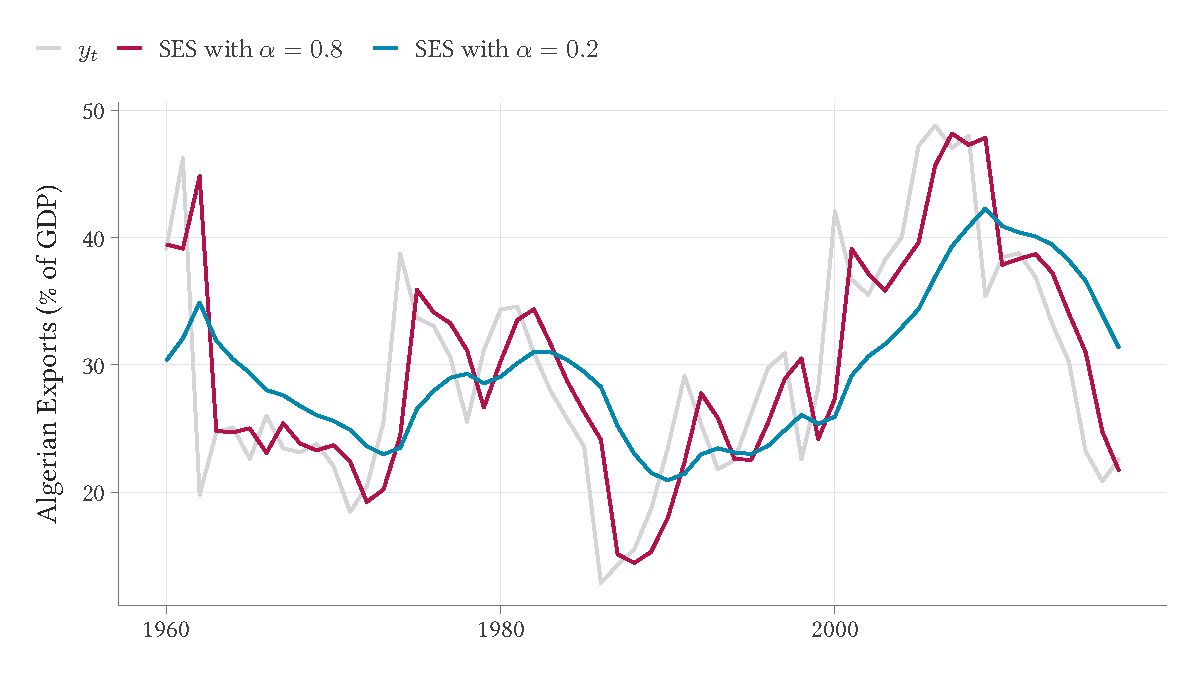
\includegraphics[width = 0.9\textwidth]{figures/algerian_exports_ses_alphas}
  \end{center}
\end{frame}

\begin{frame}{Algerian Exports Example}
  \begin{columns}[T]
    \hfill
    \begin{column}{.2\textwidth}
      \begin{table}
\centering
\begin{tblr}[         %% tabularray outer open
]                     %% tabularray outer close
{                     %% tabularray inner open
colspec={Q[]Q[]},
}                     %% tabularray inner close
\toprule
$\alpha$ & MSPE \\ \midrule %% TinyTableHeader
0.05 & 4237.193 \\
0.15 & 3543.732 \\
0.25 & 2967.187 \\
0.35 & 2565.885 \\
0.45 & 2311.215 \\
\bottomrule
\end{tblr}
\end{table}

    \end{column}
    \begin{column}{.2\textwidth}
      \begin{table}
\centering
\begin{tblr}[         %% tabularray outer open
]                     %% tabularray outer close
{                     %% tabularray inner open
colspec={Q[]Q[]},
}                     %% tabularray inner close
\toprule
$\alpha$ & MSPE \\ \midrule %% TinyTableHeader
0.55 & 2153.324 \\
0.65 & 2058.575 \\
0.75 & 2008.838 \\
0.85 & 1995.456 \\
0.95 & 2014.927 \\
\bottomrule
\end{tblr}
\end{table}

    \end{column}
    \hfill
    \begin{column}{.5\textwidth}
      The MSPE appears to minimized around $\alpha = 0.85$. Indeed the optimal is $\hat{\alpha} = 0.840$
    \end{column}
  \end{columns}
\end{frame}

\begin{frame}[fragile]{SES  in R}
  The \texttt{forecast} package makes this much simpler:
  
  \bigskip
  \vspace*{-\bigskipamount}
  \begin{codeblock}
library(forecast)
ses(y, alpha = 0.7) # optimally selects l_0
ses(y)              # optimally selects alpha and l_0
  \end{codeblock}
\end{frame}



\subsection{Trends and Seasonality with SES}

\begin{frame}{Trends}
  The \emph{simple} exponential smoothing method can fail when the data has long-term trends
  \begin{itemize}
    \item When $\alpha$ is smaller, we lean more on observations from the past (when the trend was lower)
  \end{itemize}

  \bigskip
  For example, let's look at smoothing US GDP estimates
\end{frame}

\imageframe{figures/gdp.pdf}
\imageframe{figures/gdp_ses_alphas.pdf}

\begin{frame}{Simple Exponential Smoothing and Trends}
  Since GDP is consistently trending upwards, old values of $y_{t-k}$ are systematically lower
  \begin{itemize}
    \item Lower values of $\alpha$ will put more weight on older values, hence $\hat{y}_t$ being systematically too low
  \end{itemize}

  \bigskip
  SES will also miss seasonal trends
  \begin{itemize}
    \item E.g. consider retail employment which is systematically higher around the end of the year
  \end{itemize}
\end{frame}

\imageframe{figures/retail.pdf}
\imageframe{figures/retail_ses_alphas.pdf}

% \begin{frame}{Holt-Winters method}
%   Once again, we face this problem with these methods that we focus mainly on using recent observations in terms of $t$
%   \begin{itemize}
%     \item This ignores \emph{trends} and \emph{seasonality}
%   \end{itemize}
% 
%   \bigskip
%   The \alert{Holt-Winters} method is a more advanced method that allows for (1) repeated seasonality (year-over-year) and (2) smoothly-evolving trends 
%   \begin{itemize}
%     \item Allows us to not `overfit' short term fluctuations as much by learning something about general longer-run trends
%   \end{itemize}
% \end{frame}

\begin{frame}{Simple Exponential Smoothing Method}
  Our forecast was based on
  \begin{align*}
    \text{Forecast equation:} && \hat{y}_{T+h} &= \tcbhighmath[colback = bgRaspberry]{\ell_{T}} \\[2mm]
    \text{Level equation:}    && \ell_{t} &= \alpha y_{t} + (1 - \alpha)(\ell_{t-1}) 
  \end{align*}
  
  \bigskip
  The level equation updates with new observations with weight determined by $\alpha$
\end{frame}

\begin{frame}{Holt Method for Trends}
  The Holt method adds in a trend term $b_t$ that also will be updating with observations
  \begin{align*}
    \text{Forecast equation:} && \hat{y}_{T+h} &= \tcbhighmath[colback = bgRaspberry]{\ell_{T} + hb_{T}} \\[2mm]
    \text{Level equation:}    && \ell_{t} &= \alpha y_{t} + (1 - \alpha)(\ell_{t-1} + b_{t-1}) \\[2mm]
    \text{Trend equation:}    && b_{t}    &= \beta(\ell_{t} - \ell_{t-1}) + (1 -\beta)b_{t-1},
  \end{align*}

  \bigskip 
  Level equation balances current $y_t$ with what we would forecast it to be $\ell_{t-1} + b_{t-1}$

  \bigskip
  Trend equation updates between the change in $\ell_t - \ell_{t-1}$ and the old trend $b_{t-1}$
\end{frame}

\imageframe{figures/usage.pdf}
\imageframe{figures/usage_ses_alphas.pdf}
\imageframe{figures/usage_ses_and_holt.pdf}

\begin{frame}[fragile]{Holt Method  in R}
  \vspace*{-\bigskipamount}
  \begin{codeblock}
library(forecast)
holt(y, alpha = 0.7, beta = 0.15)
holt(y) # optimally selects alpha and beta
  \end{codeblock}
\end{frame}

\begin{frame}{Choosing $\alpha$ and $\beta$ optimally}
  Similar to before, we can estimate the optimal $\alpha$ and $\beta$ by minimizing the MSPE over \emph{both} $\alpha$ and $\beta$

  \begin{itemize}
    \item Will tend to select high $\alpha$ and small $\beta$ for trending data. 
  \end{itemize}
\end{frame}

\begin{frame}{Trends and Forecasting}
  \vspace*{-\bigskipamount}
  $$
    \hat{y}_{T+h} = \ell_{T} + \tcbhighmath[colback = bgRaspberry]{h b_{T}}
  $$
  
  The Holt method forecasts using a $h$ time period extension of the slope $b_T$
  \begin{itemize}
    \item Often times we expect the trend to go away (can not go up forever)
  \end{itemize}

  \bigskip
  We can add a \alert{dampening} parameter to our model to address this
\end{frame}

\begin{frame}{Dampening in Holt method}
  \begin{align*}
    \text{Forecast equation:} && \hat{y}_{T+h} &= \ell_{T} + (\phi+\phi^2 + \dots + \phi^{h}) b_{T} \\[2mm]
    \text{Level equation:}    && \ell_{t} &= \alpha y_{t} + (1 - \alpha)(\ell_{t-1} + \phi b_{t-1}) \\[2mm]
    \text{Trend equation:}    && b_{t}    &= \beta(\ell_{t} - \ell_{t-1}) + (1 -\beta) \phi b_{t-1}
  \end{align*}

  \bigskip
  Same idea, but now $\phi$ `dampens' the trend $b_t$
  \begin{itemize}
    \item Add \texttt{damped = TRUE} to \texttt{holt} call to add a dampening parameter to the model
  \end{itemize}
\end{frame}

\imageframe{figures/usage_forecast_ses.pdf}
\imageframe{figures/usage_forecast_holt.pdf}
\imageframe{figures/usage_forecast_holt_damped.pdf}
\imageframe{figures/usage_forecast_all_3.pdf}


\begin{frame}{Holt-Winters Method}
  I will save you the details (FPP3 Section 8.3), but you can also adapt the Holt method to add seasonality to the pattern 

  \bigskip
  Use function \texttt{hw} just like \texttt{ses} and \texttt{holt}
  \begin{itemize}
    \item Also includes an option for \texttt{damped}
  \end{itemize}
\end{frame}



\end{document}
